\documentclass[12pt]{article}

% Packages.

% Writing.
\usepackage[utf8]{inputenc}
\usepackage[english]{babel}
\usepackage{enumitem} % Enumerate using letters (\begin{description}[\alph]).

\usepackage{subfiles}

% Drawing, tables and images.
\usepackage{graphicx}
\usepackage{subfigure}
\usepackage{float} % Help in table and image positioning.
\usepackage{qtree}
\usepackage{tikz}


% Math.
\usepackage{mathtools} % Overbrackets.
\usepackage{amsmath} % Symbols.
\usepackage{amsthm} % Theorems.
\usepackage{amssymb} % Mathbb{}.
\usepackage{stmaryrd} % Brackets.
\usepackage{semantic}
\usepackage{relsize}

% Exercises.
\usepackage{exercise, chngcntr}
\counterwithin{Exercise}{section}
\counterwithin{Answer}{section}

% New commands.

% Theorems.
\newtheorem{Osservazione}{Osservazione}[section]
\newtheorem{Definizione}{Definizione}[section]
\newtheorem{Teorema}{Teorema}[section]
\newtheorem{Lemma}{Lemma}[section]
\newtheorem{Corollario}{Corollario}[section]
\newtheorem{thm}{Thm}[section]

\newcommand*{\uepsilon}{\underline{\epsilon}}
\newcommand*{\uempty}{\underline{\varnothing}}
\newcommand*{\ucdot}{\mathbin{\underline{\mathord{\cdot}}}}
\newcommand*{\lpar}{\underline{(}}
\newcommand*{\rpar}{\underline{)}}
\newcommand*{\ersem}[1]{\llbracket #1 \rrbracket}
\newcommand*{\bigersem}[1]{\bigl\llbracket #1 \bigr\rrbracket}
\newcommand*{\match}{\mathrel{\lessdot}}
\newcommand*{\nmatch}{\mathrel{\not\!\!\lessdot}}
\newcommand*{\Nset}{\mathbb{N}}
\newcommand*{\Rset}{\mathbb{R}}
\newcommand*{\defeq}{\mathrel{:=}}
\newcommand*{\sseq}{\subseteq}
\newcommand*{\ttt}{\texttt}
\newcommand*{\card}[1]{\lvert #1 \rvert}
\newcommand*{\powset}[1]{\wp(#1)}
\newcommand*{\powsetf}[1]{\wp_{f}(#1)}
\newcommand*{\st}{\mathrel{.}} % Such that, to be used with \exists.
\newcommand*{\itc}{\mathrel{:}} % It is the case that, to be used with \forall.
\newcommand*{\hd}{\hat{\delta}}
\newcommand*{\cd}{\check \delta}
\newcommand*{\ep}{\epsilon}
\newcommand*{\epstep}{\epsilon\text{-step}}
\newcommand*{\epclos}{\epsilon\text{-closure}}
\newcommand*{\rel}{\mathrel R}
\newcommand*{\nrel}{\mathrel{\not\!\!R}}
\newcommand*{\qt}{q_{\varnothing}}
\newcommand*{\ra}{\rightarrow}
\newcommand*{\grder}{\stackrel{G}{\Rightarrow}}
\newcommand*{\grderp}{\stackrel{G'}{\Rightarrow}}
\newcommand*{\grders}{\stackrel{G''}{\Rightarrow}}
\newcommand*{\grdef}{\mathrel{\mathord{:}\mathord{:}\mathord{=}}}
\newcommand*{\gralt}{\mathrel{\mid}}
\newcommand*{\defpar}{\rightarrowtail}
\newcommand*{\compl}[1]{\overline{#1}}
\newcommand*{\qmarrow}{\stackrel{\text{\larger{\textbf{?}}}}{\Longrightarrow}}
\newcommand*{\twodots}{\mathrel{. \, .}}

\def\checkmark{\tikz\fill[scale=0.4](0,.35) -- (.25,0) -- (1,.7) -- (.25,.15)
  -- cycle;}

\title
{
  The Room Walk:\\
  a constraint optimization problem
}

\author{
  \texttt{federico.serafini@studenti.unipr.it}
}

\date{30/08/2022}

\begin{document}

\begin{titlepage}
  \clearpage\maketitle
  \thispagestyle{empty}
\end{titlepage}


\tableofcontents
\newpage

\section{The problem}

Let us consider a $n \times n$ shaped room, with access door $I$ located at cell
$(1, 1)$ and exit door $O$ located at cell $(n, n)$ (see picture, with $n = 6$).
The room can contain $1 \times k$ or $k \times 1$ walls. The allowed moves are either horizontal of vertical.
The problem is to identify a (the) minimal length path from $I$ to $O$. As tie
breaking for length, less turns in the path are preferred. If necessary, you
can solve the corresponding decision problem based on path length.

\begin{figure}[H]
  \begin{center}
    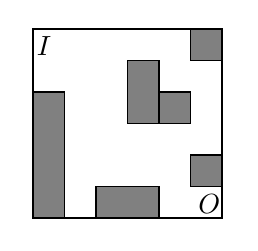
\begin{tikzpicture}[xscale=0.4,yscale=0.4]
      %\draw (0,0) grid (6,6);
      \draw (0,0) -- (6,0) -- (6,6) -- (0,6) -- (0,0);
      \draw [fill=gray] (0,0) rectangle (1,4);
      \draw [fill=gray] (3,5) rectangle (4,3);
      \draw [fill=gray] (2,0) rectangle (4,1);
      \draw [fill=gray] (5,1) rectangle (6,2);
      \draw [fill=gray] (4,3) rectangle (5,4);
      \draw [fill=gray] (5,5) rectangle (6,6);
      \draw  (5.6,0.45) node  {$O$};
      \draw  (0.35,5.45) node  {$I$};
    \end{tikzpicture}
  \end{center}
  \caption{$6 \times 6$ room} \label{room}
\end{figure}

\section{Modeling}
A matrix is the best-suitable data structure for room and path representation.
Instead of using a single and more complex matrix to represent both of them,
two different but simpler matrix are used and the relations between them are
built using constraints.

\subsection{Parameters}
\begin{itemize}
  \item
  Room size $n \in \Nset$.
  \item
  Room $R$ is a $n \times n$ binary matrix,
  where $\forall i, j \in [1 \twodots n] \itc$
    \[
    R[i, j] =
    \begin{cases}
      1,
        &\text{if there is a wall};\\
      0,
        &\text{otherwise.}
    \end{cases}
    \]
  $R$ is randomly generated  using a C program and all of its values
  are set and defined (no decision variables in $R$, it is an input parameter
  of our model).
\end{itemize}

\subsection{Variables}
\begin{itemize}
  \item
  Path $P$ is a $n+2 \times n+2$ binary matrix,
  where $\forall i, j \in [1 \twodots n+2] \itc$
    \[
    P[i, j] =
    \begin{cases}
      1,
        &\text{if it is a step of the path};\\
      0,
        &\text{otherwise.}
    \end{cases}
    \]
    $P$ contains the decision variables of our model and its
    increased size wrt $R$ is due to the zero-padding constraints,
    needed to simplify a lot the neighborhood exploration (see later).
\end{itemize}

\subsection{Constraints}

\subsubsection{Static constraints}
In this document, a constraint is called \emph{static} if all the information
needed for its evaluation are available at ``compile time".
\begin{itemize}
  \item
  Zero padding (first row, first column, last row, last column):
  \begin{align*}
    &\forall j \in [1 \twodots n+2] \itc P[1,j] = 0 \\
      &\wedge \\
    &\forall i  \in [1 \twodots n+2] \itc P[i,1] = 0 \\
      &\wedge\\
    &\forall j \in [1 \twodots n+2] \itc P[n+2,j] = 0 \\
      &\wedge\\
    &\forall i \in [1 \twodots n+2] \itc P[i,n+2] = 0.
  \end{align*}
  \item
  Enter and exit cells (both must be part of the path):
  \[
    P[2,2] = 1 \wedge P[n+1, n+1] = 1.
  \]
  \item
  Avoid walls (if there is a wall then the path can not step over it):
  \[
    \forall i, j \in [1 \twodots n] \itc R[i, j] > 0
    \Longrightarrow
    P[i+1,j+1] = 0.
  \]
\end{itemize}
Taking example room in Fig.~\ref{room} as input matrix $R$,
after the static constraint evaluation, the matrix $P$ looks like the following:
\begin{figure}[H]
  \begin{center}
    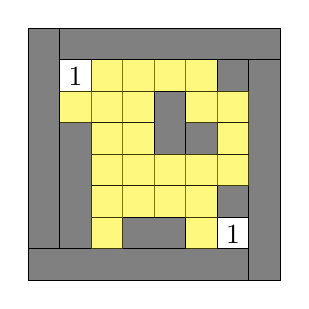
\begin{tikzpicture}[xscale=0.4,yscale=0.4]
      \draw (0,0) grid (8,8);
      \draw (0,0) -- (8,0) -- (8,8) -- (0,8) -- (0,0);
      \draw [fill=gray] (1,1) rectangle (2,5);
      \draw [fill=gray] (4,6) rectangle (5,4);
      \draw [fill=gray] (3,1) rectangle (5,2);
      \draw [fill=gray] (6,2) rectangle (7,3);
      \draw [fill=gray] (5,4) rectangle (6,5);
      \draw [fill=gray] (6,6) rectangle (7,7);
      \draw [fill=gray] (0,0) rectangle (1,8);
      \draw [fill=gray] (0,7) rectangle (8,8); % First row padding.
      \draw [fill=gray] (0,0) rectangle (1,8); % First column padding.
      \draw [fill=gray] (0,0) rectangle (7,1); % Last row padding.
      \draw [fill=gray] (7,0) rectangle (8,7); % Last column padding.
      \draw (1.5, 6.45) node {$1$};
      \draw (6.5, 1.45)  node {$1$};
      \draw [fill=yellow, opacity=0.5] (2, 7) rectangle (6,6);
      \draw [fill=yellow, opacity=0.5] (1, 6) rectangle (4,5);
      \draw [fill=yellow, opacity=0.5] (2, 5) rectangle (4,4);
      \draw [fill=yellow, opacity=0.5] (2, 4) rectangle (7,3);
      \draw [fill=yellow, opacity=0.5] (2, 3) rectangle (6,2);
      \draw [fill=yellow, opacity=0.5] (2, 2) rectangle (3,1);
      \draw [fill=yellow, opacity=0.5] (5, 1) rectangle (6,2);
      \draw [fill=yellow, opacity=0.5] (5, 6) rectangle (7,5);
      \draw [fill=yellow, opacity=0.5] (6, 5) rectangle (7,4);
    \end{tikzpicture}
  \end{center}
  \caption{Matrix $P$ after static constrain evaluation}
\end{figure}
Where:
\[
  P[i,j]=
  \begin{cases}
    0,
      &\text{if cell is gray;}\\
    0 \vee 1,
      &\text{if cell is yellow (free variable);}\\
    1,
      &\text{otherwise}.
  \end{cases}
\]
\subsubsection{Dynamic constraints}
In this document, a constraint is called \emph{dynamic} if it introduces
relations between variables whose compile-time evaluation is not possible,
for example:
constraints needed to connect the enter point with the exit point in order to
create a path between them.
\begin{itemize}
  \item
  Neighborhood for enter and exit cells (exactly one neighbor each):
  \[
    P[2,3] + P[3,2] = 1 \wedge P[n+1,n] + P[n,n+1] = 1;
  \]
  \item
  Neighborhood for all the other cells in the path (exactly two neighbors each):
  \begin{align*}
    &\forall i,j \in [2 \twodots n+1] \itc
    P[i, j] > 0 \Longrightarrow\\
    &\Bigl(
    \neg \bigl( (i = 2 \wedge j = 2) \vee ( i = n+1 \wedge j = n+1) \bigr)
    \Longrightarrow \\
    & P[i-1,j] + P[i,j-1] + P[i+1,j] + P[i,j+1] = 2
    \Bigr).
  \end{align*}
\end{itemize}

\subsubsection{Length and turns}
Thanks to the modeling decisions taken so far, the computation of length and
number of turns in the path are straight forward.
\begin{itemize}
  \item Lenght $l \in \Nset$:
  \[
    l = \sum_{i, j = 2}^{n+1} P[i,j].
  \]
  \item
  Turn detection is performed using a convolution operation over the
  non-padded section of the matrix $P$, with a $2 \times 2$ filter full
  of ones.

  The result of each filter application, is encoded in the $n-1 \times n-1$
  binary matrix $tc$ (turn
  counter).
  $\forall i, j \in [2 \twodots n] \itc$
  \[
    tc[i-1,j-1] =
    \begin{cases}
      1,
        &\text{if } \sum_{s, t = 0}^{1} P[i+s,j+t] \geq 3;\\
      0,
        &\text{otherwise.}
    \end{cases}
  \]
    \begin{figure}[H]
    \begin{center}
      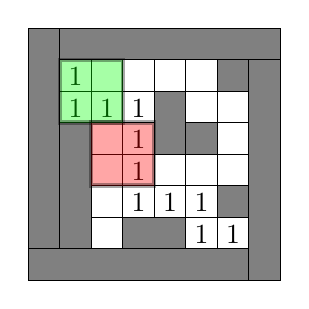
\begin{tikzpicture}[xscale=0.4,yscale=0.4]
        \draw (0,0) grid (8,8);
        \draw (0,0) -- (8,0) -- (8,8) -- (0,8) -- (0,0);
        \draw [fill=gray] (1,1) rectangle (2,5);
        \draw [fill=gray] (4,6) rectangle (5,4);
        \draw [fill=gray] (3,1) rectangle (5,2);
        \draw [fill=gray] (6,2) rectangle (7,3);
        \draw [fill=gray] (5,4) rectangle (6,5);
        \draw [fill=gray] (6,6) rectangle (7,7);
        \draw [fill=gray] (0,0) rectangle (1,8);
        \draw [fill=gray] (0,7) rectangle (8,8); % First row padding.
        \draw [fill=gray] (0,0) rectangle (1,8); % First column padding.
        \draw [fill=gray] (0,0) rectangle (7,1); % Last row padding.
        \draw [fill=gray] (7,0) rectangle (8,7); % Last column padding.
        \draw (1.5, 6.45) node {$1$};
        \draw (1.5, 5.45) node {$1$};
        \draw (2.5, 5.45) node {$1$};
        \draw (3.5, 5.45) node {$1$};
        \draw (3.5, 4.45) node {$1$};
        \draw (3.5, 3.45) node {$1$};
        \draw (3.5, 2.45) node {$1$};
        \draw (4.5, 2.45) node {$1$};
        \draw (5.5, 2.45) node {$1$};
        \draw (5.5, 1.45) node {$1$};
        \draw (6.5, 1.45)  node {$1$};
        \draw [ultra thick, fill=green, opacity=0.35] (1,5) rectangle (3,7);
        \draw [ultra thick, fill=red, opacity=0.35] (2, 3) rectangle (4,5);
      \end{tikzpicture}
    \end{center}
    \caption{Turn detection in green}
  \end{figure}
  \item Turns $t \in \Nset$:
  \[
    t = \sum_{i, j = 1}^{n-1} \textit{tc}[i, j].
  \]
\end{itemize}


\subsection{Cost function minimization}
Given all the constraint discussed so far, the function $f$ to minimize is the
following:
\begin{align}
  \label{f}
  f = l^2 + t.
\end{align}
The length squared is needed to give priority to the shortest paths and then
using turns as tie breaking.
\begin{proof}
  The proof is based on the fact that $\forall \text{ path } p \text{ of length
  $l$ and turns $t$} \itc$
  \begin{align}
    \label{t}
    & 1 \leq t < l.
  \end{align}
  Let $p_1$ be a path of length $l_1$ and $t_1$
  turns.
  Let $p_2$ be a path of length $l_2 = l_1 +1$ and $t_2 < t_1$ turns.
  \begin{align*}
    f_1
      &= l_1^2 + t_1
        &\text{[\eqref{f}]}\\
      & < l_1^2 + l_1
        &\text{[\eqref{t}]}\\
      & < l_1^2 + 2l_1
        &\text{[\eqref{t}]}\\
      & < l_1^2 + 2l_1 + 1 + t_2
        &\text{[\eqref{t}]}\\
      & = (l_1 + 1)^2 + t_2\\
      & =  l_2^2 + t_2
       &\text{[$l_2 = l_1 + 1$]}\\
      &= f_2
        &\text{[\eqref{f}]}.
  \end{align*}
$f_1 < f_2$ then $p_1$ is preferred, no matter if $p_2$ has lass turns.
\end{proof}

\subsection{Additional constraints to help the search}
Constraints seen so far, together with the minimization of the cost function
$f$, are enough to find the optimal solution. However, during the search
procedure, it is possible that undesired candidate solutions are found, for
example:

\begin{figure}[H]
  \centering
  \begin{minipage}{.5\textwidth}
      \begin{center}
      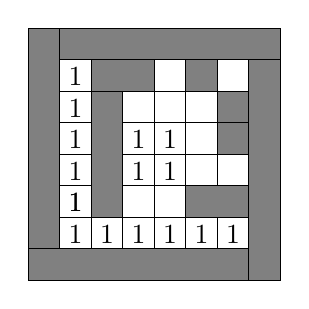
\begin{tikzpicture}[xscale=0.4,yscale=0.4]
        \draw (0,0) grid (8,8);
        \draw (0,0) -- (8,0) -- (8,8) -- (0,8) -- (0,0);
        \draw [fill=gray] (0,7) rectangle (8,8); % First row padding.
        \draw [fill=gray] (0,0) rectangle (1,8); % First column padding.
        \draw [fill=gray] (0,0) rectangle (7,1); % Last row padding.
        \draw [fill=gray] (7,0) rectangle (8,7); % Last column padding.
        \draw (1.5, 6.45) node {$1$};
        \draw (1.5, 5.45) node {$1$};
        \draw (1.5, 4.45) node {$1$};
        \draw (1.5, 3.45) node {$1$};
        \draw (1.5, 2.45) node {$1$};
        \draw (1.5, 2.45) node {$1$};
        \draw (1.5, 1.45) node {$1$};
        \draw (2.5, 1.45) node {$1$};
        \draw (3.5, 1.45) node {$1$};
        \draw (4.5, 1.45) node {$1$};
        \draw (5.5, 1.45) node {$1$};
        \draw (6.5, 1.45)  node {$1$};

        \draw (3.5, 3.45) node {$1$};
        \draw (3.5, 4.45) node {$1$};
        \draw (4.5, 3.45) node {$1$};
        \draw (4.5, 4.45)  node {$1$};

        \draw [fill=gray] (2,7) rectangle (4,6);
        \draw [fill=gray] (5,3) rectangle (7,2);
        \draw [fill=gray] (5,6) rectangle (6,7);
        \draw [fill=gray] (6,5) rectangle (7,6);
        \draw [fill=gray] (6,4) rectangle (7,5);
        \draw [fill=gray] (2,2) rectangle (3,6);
      \end{tikzpicture}
    \end{center}
  \end{minipage}%
  \begin{minipage}{.5\textwidth}
    \begin{center}
      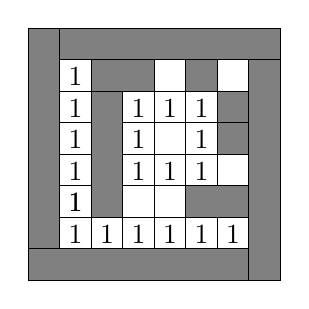
\begin{tikzpicture}[xscale=0.4,yscale=0.4]
        \draw (0,0) grid (8,8);
        \draw (0,0) -- (8,0) -- (8,8) -- (0,8) -- (0,0);
        \draw [fill=gray] (0,7) rectangle (8,8); % First row padding.
        \draw [fill=gray] (0,0) rectangle (1,8); % First column padding.
        \draw [fill=gray] (0,0) rectangle (7,1); % Last row padding.
        \draw [fill=gray] (7,0) rectangle (8,7); % Last column padding.
        \draw (1.5, 6.45) node {$1$};
        \draw (1.5, 5.45) node {$1$};
        \draw (1.5, 4.45) node {$1$};
        \draw (1.5, 3.45) node {$1$};
        \draw (1.5, 2.45) node {$1$};
        \draw (1.5, 2.45) node {$1$};
        \draw (1.5, 1.45) node {$1$};
        \draw (2.5, 1.45) node {$1$};
        \draw (3.5, 1.45) node {$1$};
        \draw (4.5, 1.45) node {$1$};
        \draw (5.5, 1.45) node {$1$};
        \draw (6.5, 1.45)  node {$1$};

        \draw (3.5, 5.45) node {$1$};
        \draw (4.5, 5.45) node {$1$};
        \draw (5.5, 5.45) node {$1$};
        \draw (5.5, 4.45) node {$1$};
        \draw (5.5, 3.45) node {$1$};
        \draw (3.5, 3.45) node {$1$};
        \draw (3.5, 4.45) node {$1$};
        \draw (4.5, 3.45) node {$1$};

        \draw [fill=gray] (2,7) rectangle (4,6);
        \draw [fill=gray] (5,3) rectangle (7,2);
        \draw [fill=gray] (5,6) rectangle (6,7);
        \draw [fill=gray] (6,5) rectangle (7,6);
        \draw [fill=gray] (6,4) rectangle (7,5);
        \draw [fill=gray] (2,2) rectangle (3,6);
      \end{tikzpicture}
    \end{center}
  \end{minipage}
  \caption{$2 \times 2$ and $3 \times 3$ squares}
\end{figure}
Solution containing this kinds of polygons will be automatically discarded since
they are incrementing the cost function value but, to speed up the search
procedure, constraints can be added.
\begin{itemize}
  \item
  Avoid $2 \times 2$ squares:
  \[
    \forall i, j \in [2 \twodots n] \itc \sum_{s, t = 0}^{1} P[i+s,j+t] \leq 3.
  \]
  \item
  Avoid $3 \times 3$ squares (a zero cell that is not a wall has at  most two
  neighbors):
  \begin{align*}
    &\forall i, j \in [2 \twodots n+1] \itc (P[i,j] = 0 \wedge R[i-1,j-1] = 0)
    \Longrightarrow\\
    &P[i-1,j] + P[i,j-1] + P[i+1,j] + P[i,j+1] \leq 2.
  \end{align*}

  \item
  Avoid $4 \times 4$ squares (a $2 \times 2$ square of zeros without walls
  has at most 4 neighbors):
  \begin{align*}
    &\forall i, j \in [2 \twodots n+1] \itc \\
    &\sum_{s, t = 0}^{1} P[i+s,j+t] + R[i+s-1,j+t-1] = 0
    \Longrightarrow \\
    &P[i-1,j] + P[i-1,j+1] + P[i,j+2] + P[i+1,j+2] +\\
    &P[i+2,j] + P[i+2,j+1] + P[i,j-1] + P[i+1,j-1] \leq 4.
  \end{align*}
\end{itemize}

Note that there are also other polygons that can be generated and,
as a future work, more constraints should be added in order to handle them:
\begin{figure}[H]
  \begin{center}
    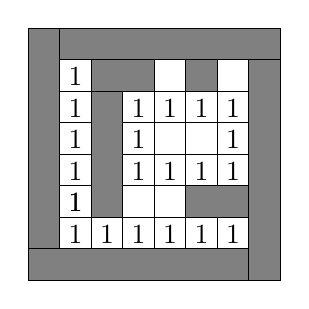
\begin{tikzpicture}[xscale=0.4,yscale=0.4]
      \draw (0,0) grid (8,8);
      \draw (0,0) -- (8,0) -- (8,8) -- (0,8) -- (0,0);
      \draw [fill=gray] (0,7) rectangle (8,8); % First row padding.
      \draw [fill=gray] (0,0) rectangle (1,8); % First column padding.
      \draw [fill=gray] (0,0) rectangle (7,1); % Last row padding.
      \draw [fill=gray] (7,0) rectangle (8,7); % Last column padding.
      \draw (1.5, 6.45) node {$1$};
      \draw (1.5, 5.45) node {$1$};
      \draw (1.5, 4.45) node {$1$};
      \draw (1.5, 3.45) node {$1$};
      \draw (1.5, 2.45) node {$1$};
      \draw (1.5, 2.45) node {$1$};
      \draw (1.5, 1.45) node {$1$};
      \draw (2.5, 1.45) node {$1$};
      \draw (3.5, 1.45) node {$1$};
      \draw (4.5, 1.45) node {$1$};
      \draw (5.5, 1.45) node {$1$};
      \draw (6.5, 1.45)  node {$1$};

      \draw (3.5, 5.45) node {$1$};
      \draw (4.5, 5.45) node {$1$};
      \draw (5.5, 5.45) node {$1$};
      \draw (6.5, 5.45) node {$1$};
      \draw (6.5, 4.45) node {$1$};
      \draw (6.5, 3.45) node {$1$};
      \draw (5.5, 3.45) node {$1$};
      \draw (3.5, 3.45) node {$1$};
      \draw (3.5, 4.45) node {$1$};
      \draw (4.5, 3.45) node {$1$};

      \draw [fill=gray] (2,7) rectangle (4,6);
      \draw [fill=gray] (5,3) rectangle (7,2);
      \draw [fill=gray] (5,6) rectangle (6,7);
      \draw [fill=gray] (2,2) rectangle (3,6);
    \end{tikzpicture}
  \end{center}
  \caption{$3 \times 4$ rectangle}
\end{figure}

\newpage

\section{MiniZinc implementation}
The formalization of the model discussed so far can be 1:1 translated into an
effective MiniZinc program.
In addition, MiniZinc allows to specify which search strategy the solver should
follow, this is because for combinatorial problems some search strategies
could be more effective than others.
For this particular problem, finding the better strategy is not trivial:
the effectiveness of a search stategy really depends on the shape of the room
that is randomly generated.

\subsection{Search strategy}
The strategy listed below achieves good performance with a fairly large and
varied sample of rooms.
\begin{itemize}
  \item
  Variables:
  as the key of our problem, it is reasonable to start the search selecting
  variables from $P$,
  since the values of $l, tc$ and $t$ are function of it and they can be easily
  derived.
  \item
  Variable choice:
  \texttt{dom\_w\_deg} annotation selects the variable of $P$ with the
  smallest value of:
  \[
    \dfrac{\card{D}}{\text{w\_deg}},
  \]
  where $\card{D}$ is the domain size and w\_deg is the weighted degree (the
  number of times the variable has been in a constraint that caused failure
  earlier in the search), thus allowing information gathering about the room
  shape from all the different explorations.
  \item
  Constraint choice: \texttt{indomain\_min} annotation assigns to the selected
  variable its smallest domain value.

  Since $l \ll n^2$ then the number of 0 in $P$ is greater than the number of 1;
  selecting the lowest value is in general the right choice
  (reduce backtraking).
  \item
  Restart:
  a bad decisions made at the top of the search tree can take
  an exponential amount of search to undo. Restart annotation allows to restart
  the search from the top thus having a chance to make different decisions
  every time a node limit in the search tree is reached.

  With \texttt{restart\_geometric(n, 1)} the $k$-th restart has a node limit of
  $1 \times n^k$. Restart and \texttt{dom\_w\_deg} together are found to be
  very effective in finding unsatisfiability.
\end{itemize}

\section{Results}
$\forall n \in \{\, 6, 8, 10, 12, 14, 16, 18 \,\} \itc $
\begin{itemize}
  \item
  20 different room instances with $2n$ walls are randomly generated;
  \item
  20 different room instances with $n$ walls are randomly generated.
\end{itemize}
Results are plotted using a linear scale for the room size ($x$ axis) and
a logarithmic scale for the time ($y$ axis).
Fixing the room size and the number of walls, the time value that is plotted
corresponds to the maximum time that is taken between all the $20$ different
instances (time in the worst case).
\begin{figure}[H]
  \centering
  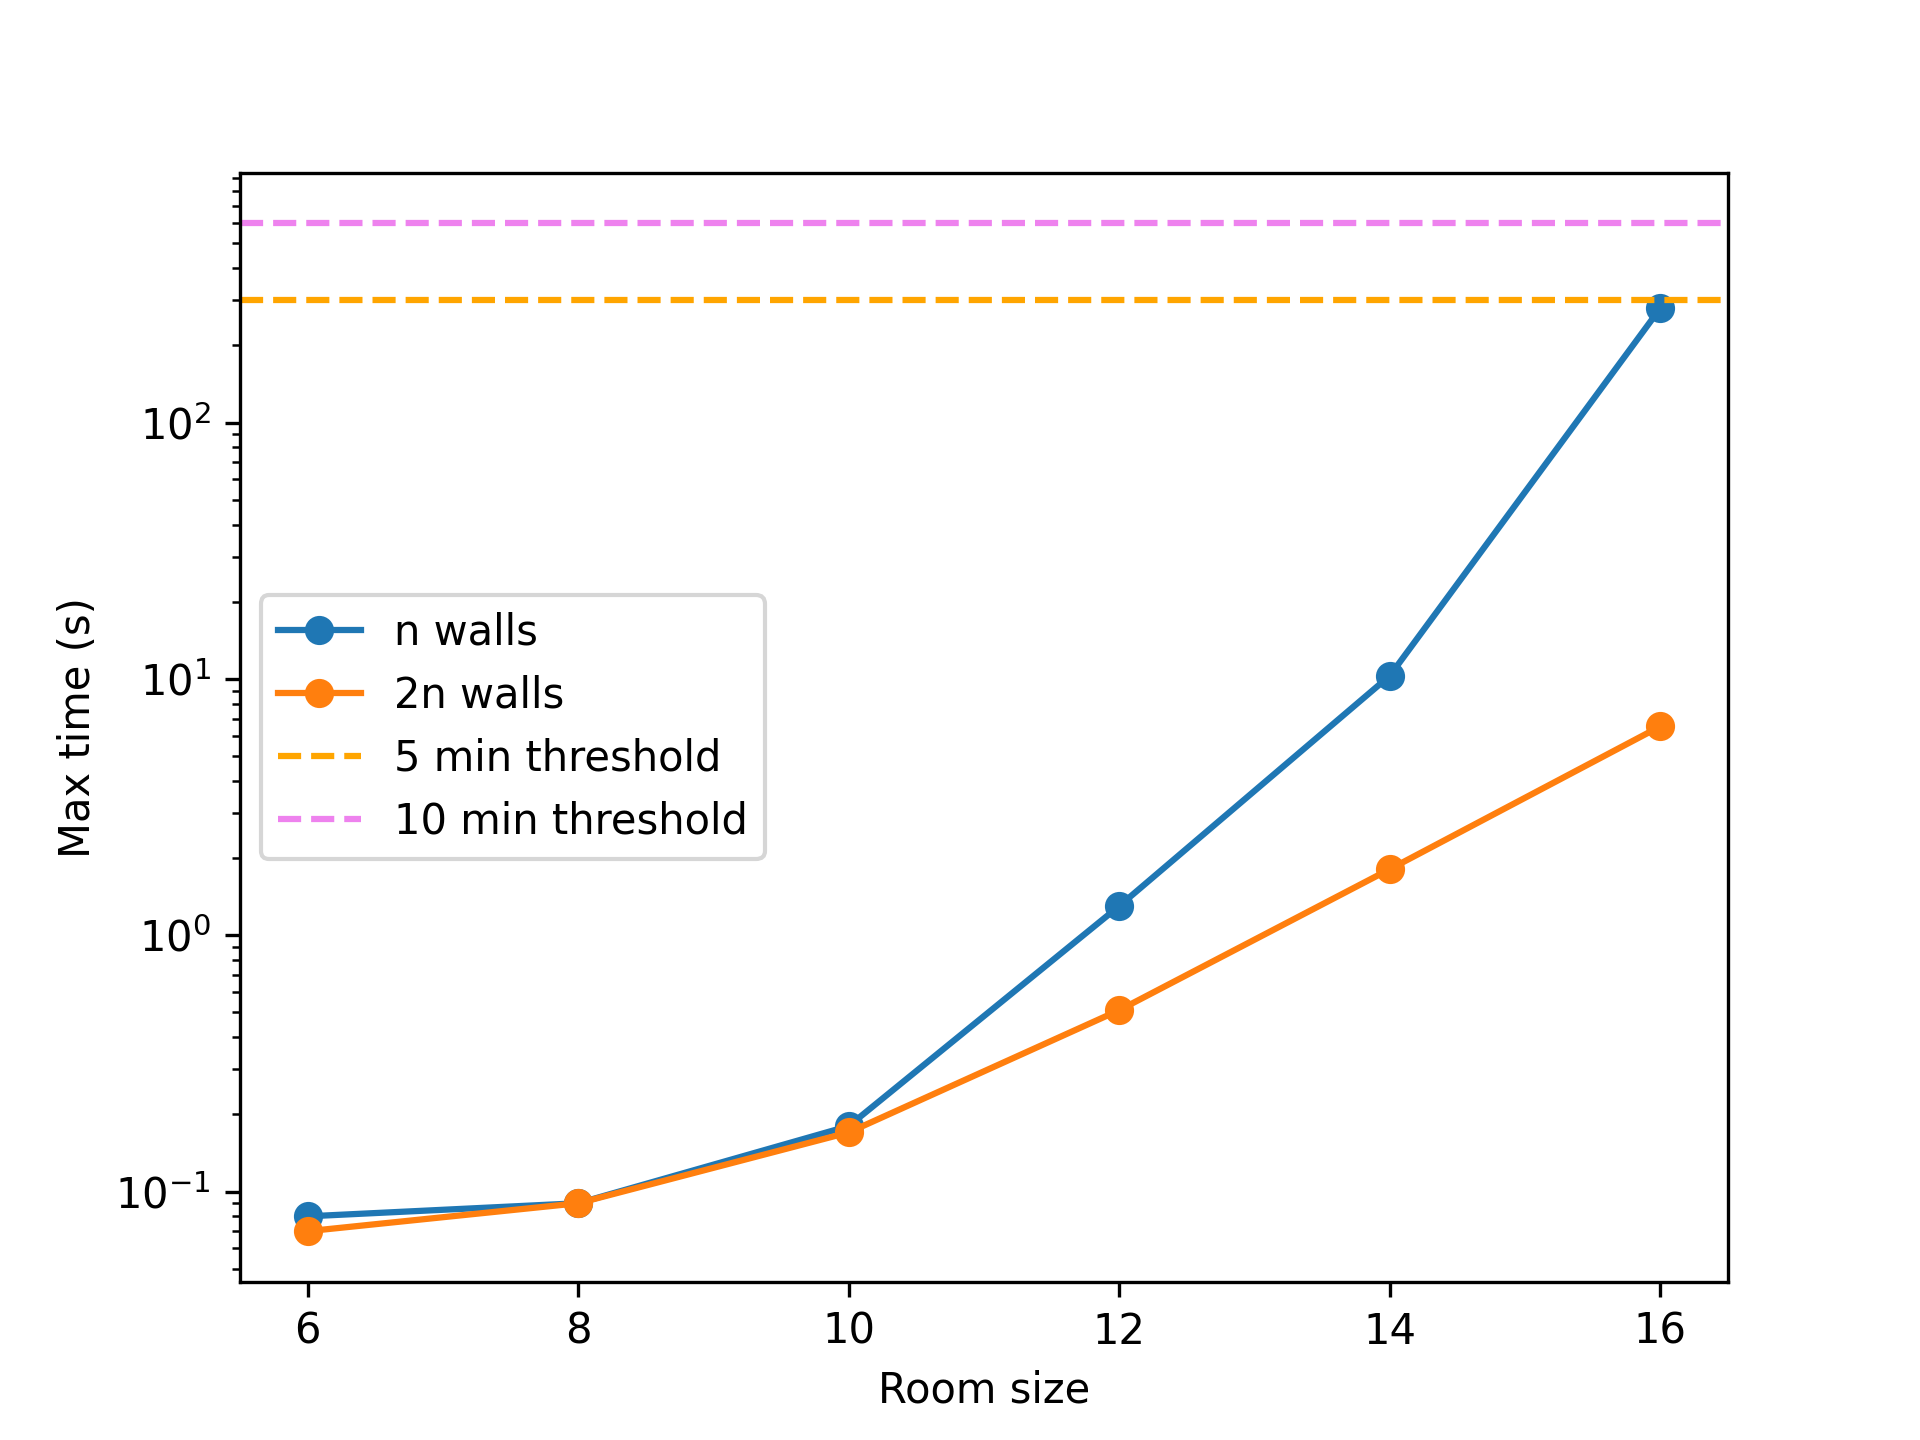
\includegraphics[width=.9\linewidth]{../Code/n-2n.png}
  \caption{$n$ and $2n$ walls}
  \label{n-2n}
\end{figure}
\begin{figure}[H]
  \centering
  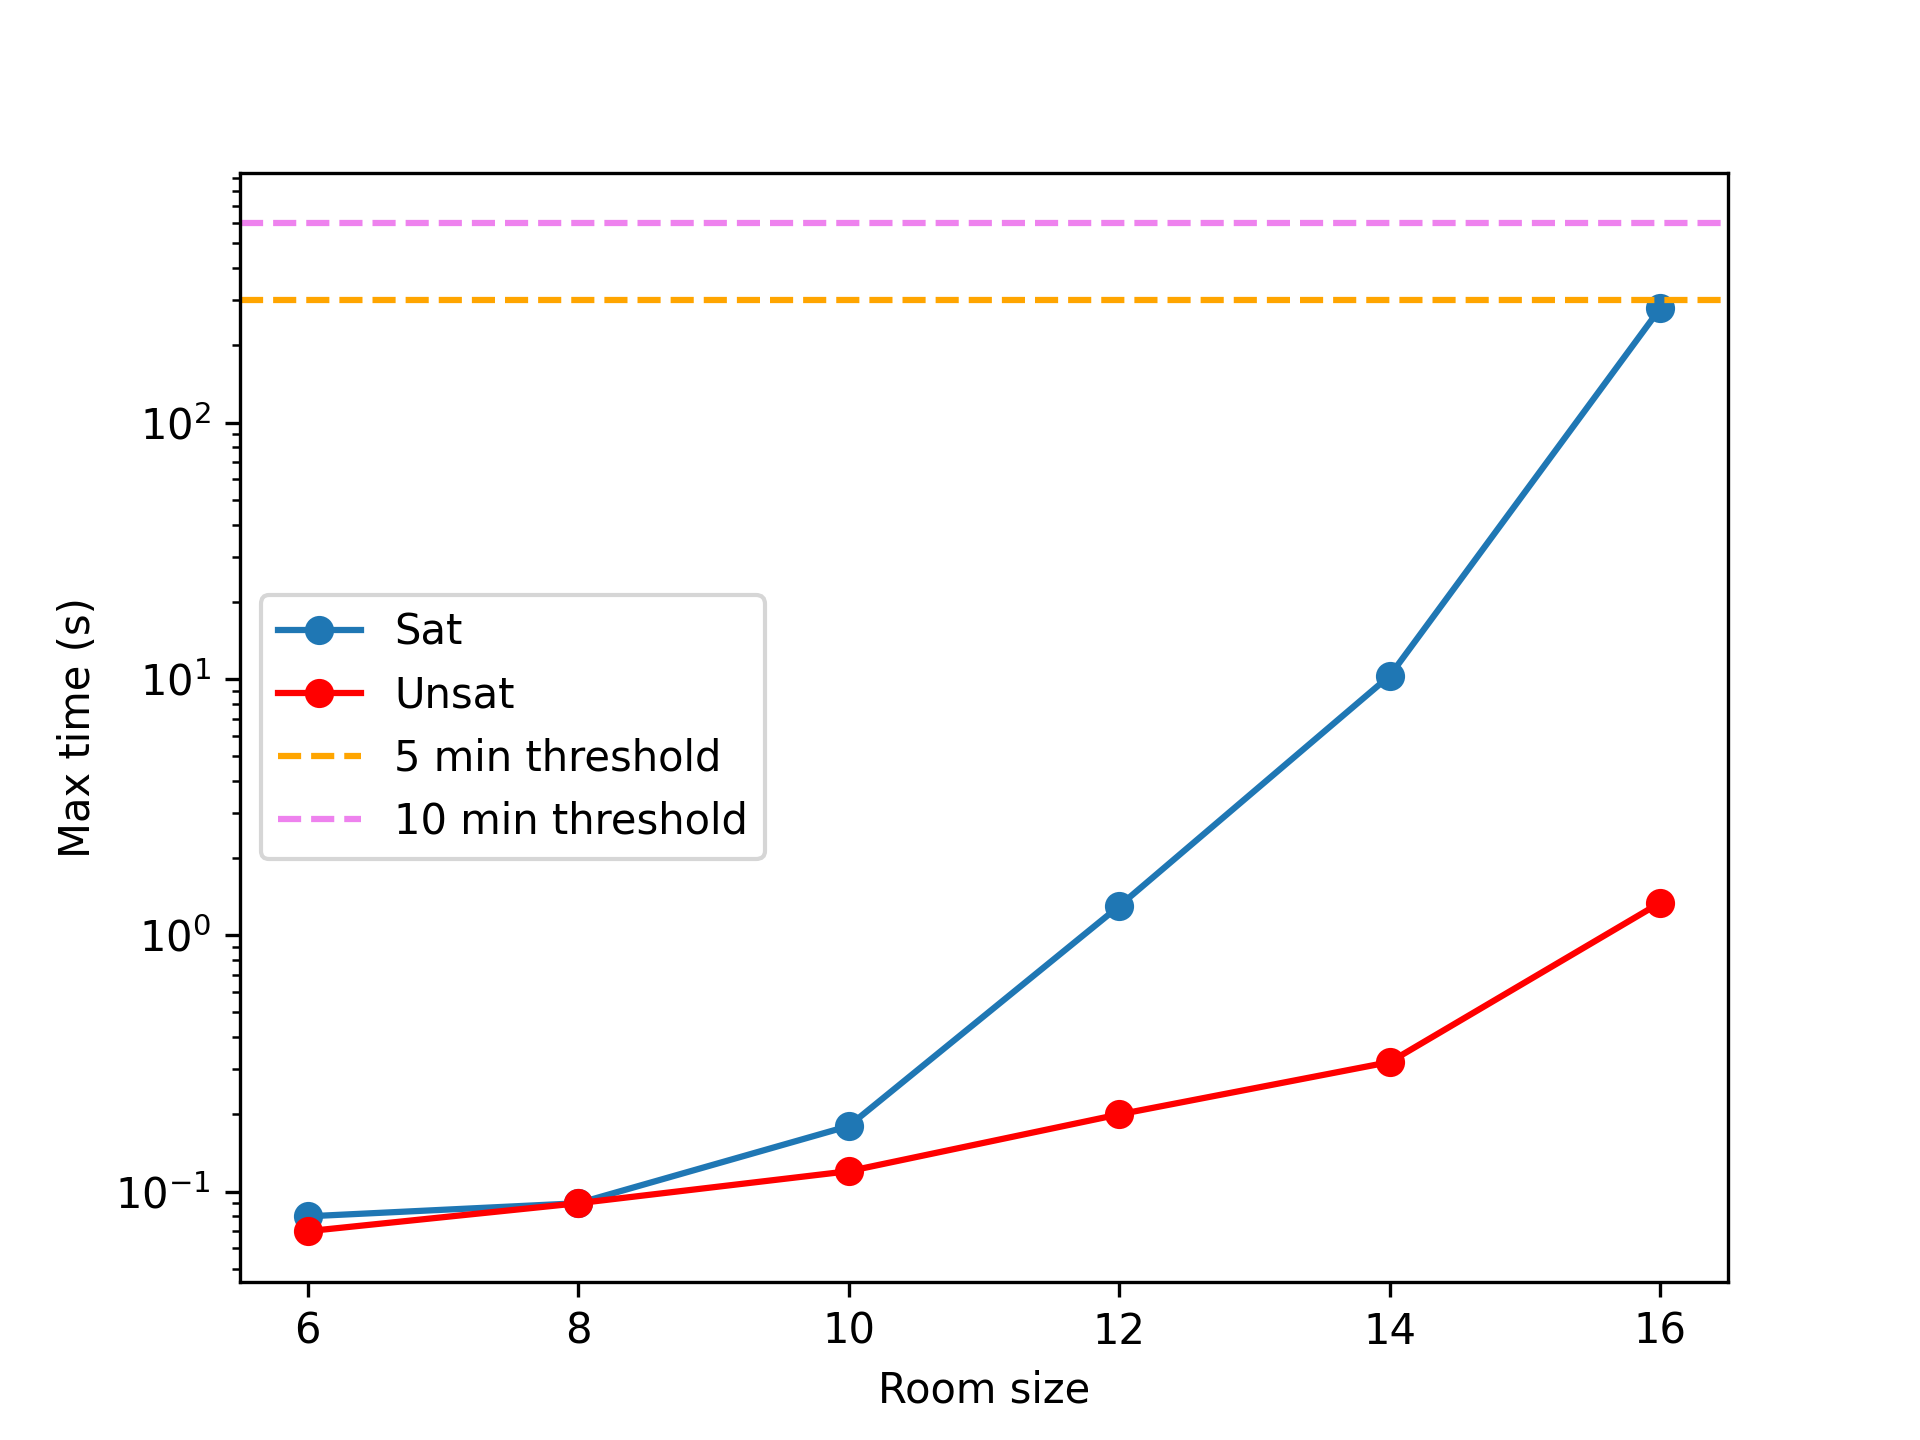
\includegraphics[width=.9\linewidth]{../Code/sat-unsat.png}
  \caption{Sat and unsat}
  \label{sat-unsat}
\end{figure}
Not considering the padding variables, there are $n^2$ decision variables
with a binary domain then, the search space has a size of $2^{n^2}$.
From the Fig.~\ref{n-2n} it is clear that finding the solution in a room with
$2n$
walls
is easier, this is because the more walls there are, the fewer decision
variables are involved (thanks to the ``avoid walls" and ``start and exit
points" static constraints):
let $w = \card{\text{wall cells}}$, then the constraint propagation, just
applying node consistency, is able to reduce the search space size to $2^{n^2
-w-2}$.

Fig.~\ref{sat-unsat} shows an appreciable feature of the model:
the ability to quickly find unsatisfiability without exploring the whole search
tree, thus allowing the final user to know in a short time if an admissible
solution exists and then, if interested,
let the solver run in order to find the optimal one.
This is feasible thanks to the model design and the search strategy that allows
a very effective constraint propagation.

Despite the logarithmic scale, in both Fig.~\ref{n-2n} and
Fig.~\ref{sat-unsat}, plotted functions seem to grow exponentially.
This is due to the fact that the ratio between the wall cells and the
variables, considering the noise introduced by randomization
and the low number of samples, can be approximated into a slowly
descending line (Fig.~\ref{ratio}). This means that the increasing the size,
the number of variables grows faster than the number of walls, resulting in  an
increase of the ``free variables" and an exponential impact on the search space
size.

\begin{figure}[H]
  \centering
  \includegraphics[width=.9\linewidth]{../Code/ratio.png}
  \caption{Ratio between wall cells and variables}
  \label{ratio}
\end{figure}

%\begin{proof}
%  Given a room $n \times n$ room $R_1$ with $n$ walls,
%  the size $k$ for each wall is randomly generated with equal probability in
%  the interval $[1 \twodots n/2]$, then, an approximation fo the average size
%  $k_1$ is the expected value of a discrete uniform distribution
%  \textit{unif}$(1, n/2)$:
%  \begin{align*}
%    k_1
%    &= \dfrac{1}{2} \Bigl( \dfrac{n}{2} +1 \Bigr).
%  \end{align*}
%  Since there are $n$ walls, then an approximation of the wall-cell count $w_1$
%  is the following:
%  \begin{align*}
%    w_1
%      & = k_1n\\
%      & = \dfrac{1}{2} \Bigl( \dfrac{n}{2} +1 \Bigr) n\\
%      & = \dfrac{n^2}{4} + \dfrac{n}{2}.
%  \end{align*}
%
%  Given a $n+2 \times n+2$ room $R_2$ with $n+2$ walls, the an approximation
%  of the wall-cell count is:
%    \begin{align*}
%    w_2
%      & = \dfrac{1}{2} \Bigl( \dfrac{n+2}{2} +1 \Bigr)n\\
%      &= \dfrac{n^2}{4} + \dfrac{2n}{2}.
%  \end{align*}
%
%  So, from size $n$ to size $n+2$, the number of wall cells added is:
%  \begin{align*}
%      w_2 - w_1
%        & = \dfrac{n^2}{4} + \dfrac{2n}{2} - \dfrac{n^2}{4} -
%        \dfrac{n}{2}\\
%        & = \dfrac{n}{2}.
%  \end{align*}
%  But, from size $n$ to size $n+2$ the number of variables added are:
%  \[
%    (n+2)^2 - n^2 = n^2 + 4n + 4 - n^2 = 4n + 4.
%  \]
%  So, the number of free variables is growing.
%\end{proof}

\end{document}
